\documentclass{beamer}
\usepackage{tikz}

\setbeamertemplate{navigation symbols}{}

\setbeamercolor{frametitle}{fg=orange}
\setbeamercolor{title}{fg=orange}
%\definecolor{tcolor}{RGB}{10,100,200}
\setbeamercolor{normal text}{fg=black}
%\setbeamercolor{normal text}{fg=RGB{} 
%\setbeamerfont{frametitle}{size=large}
\setbeamerfont{frametitle}{family=\rmfamily,shape=\itshape,size=\huge} 
\setbeamerfont{title}{family=\rmfamily,shape=\itshape,size=\huge} 

\usetheme{boxes}
\setbeamertemplate{background canvas}[vertical shading][bottom=white,top=blue!20]

\title{Cosmic Frontier at Brookhaven}

\begin{document}


%\frame{\titlepage}

\frame
{

    \frametitle{Dark Energy Survey (DES)}

    \fontsize{9}{0.8\baselineskip}

    \begin{columns}

        \begin{column}{0.5\textwidth}

            \begin{itemize}

                \item 45 papers from science verification data now published
                    or submitted

                \item 14 papers on weak lensing published or submitted

                \item Weak lensing papers are based on the shear catalogs produced
                    by Erin Sheldon (BNL)

            \end{itemize}

        \end{column}

        \begin{column}{0.5\textwidth}
            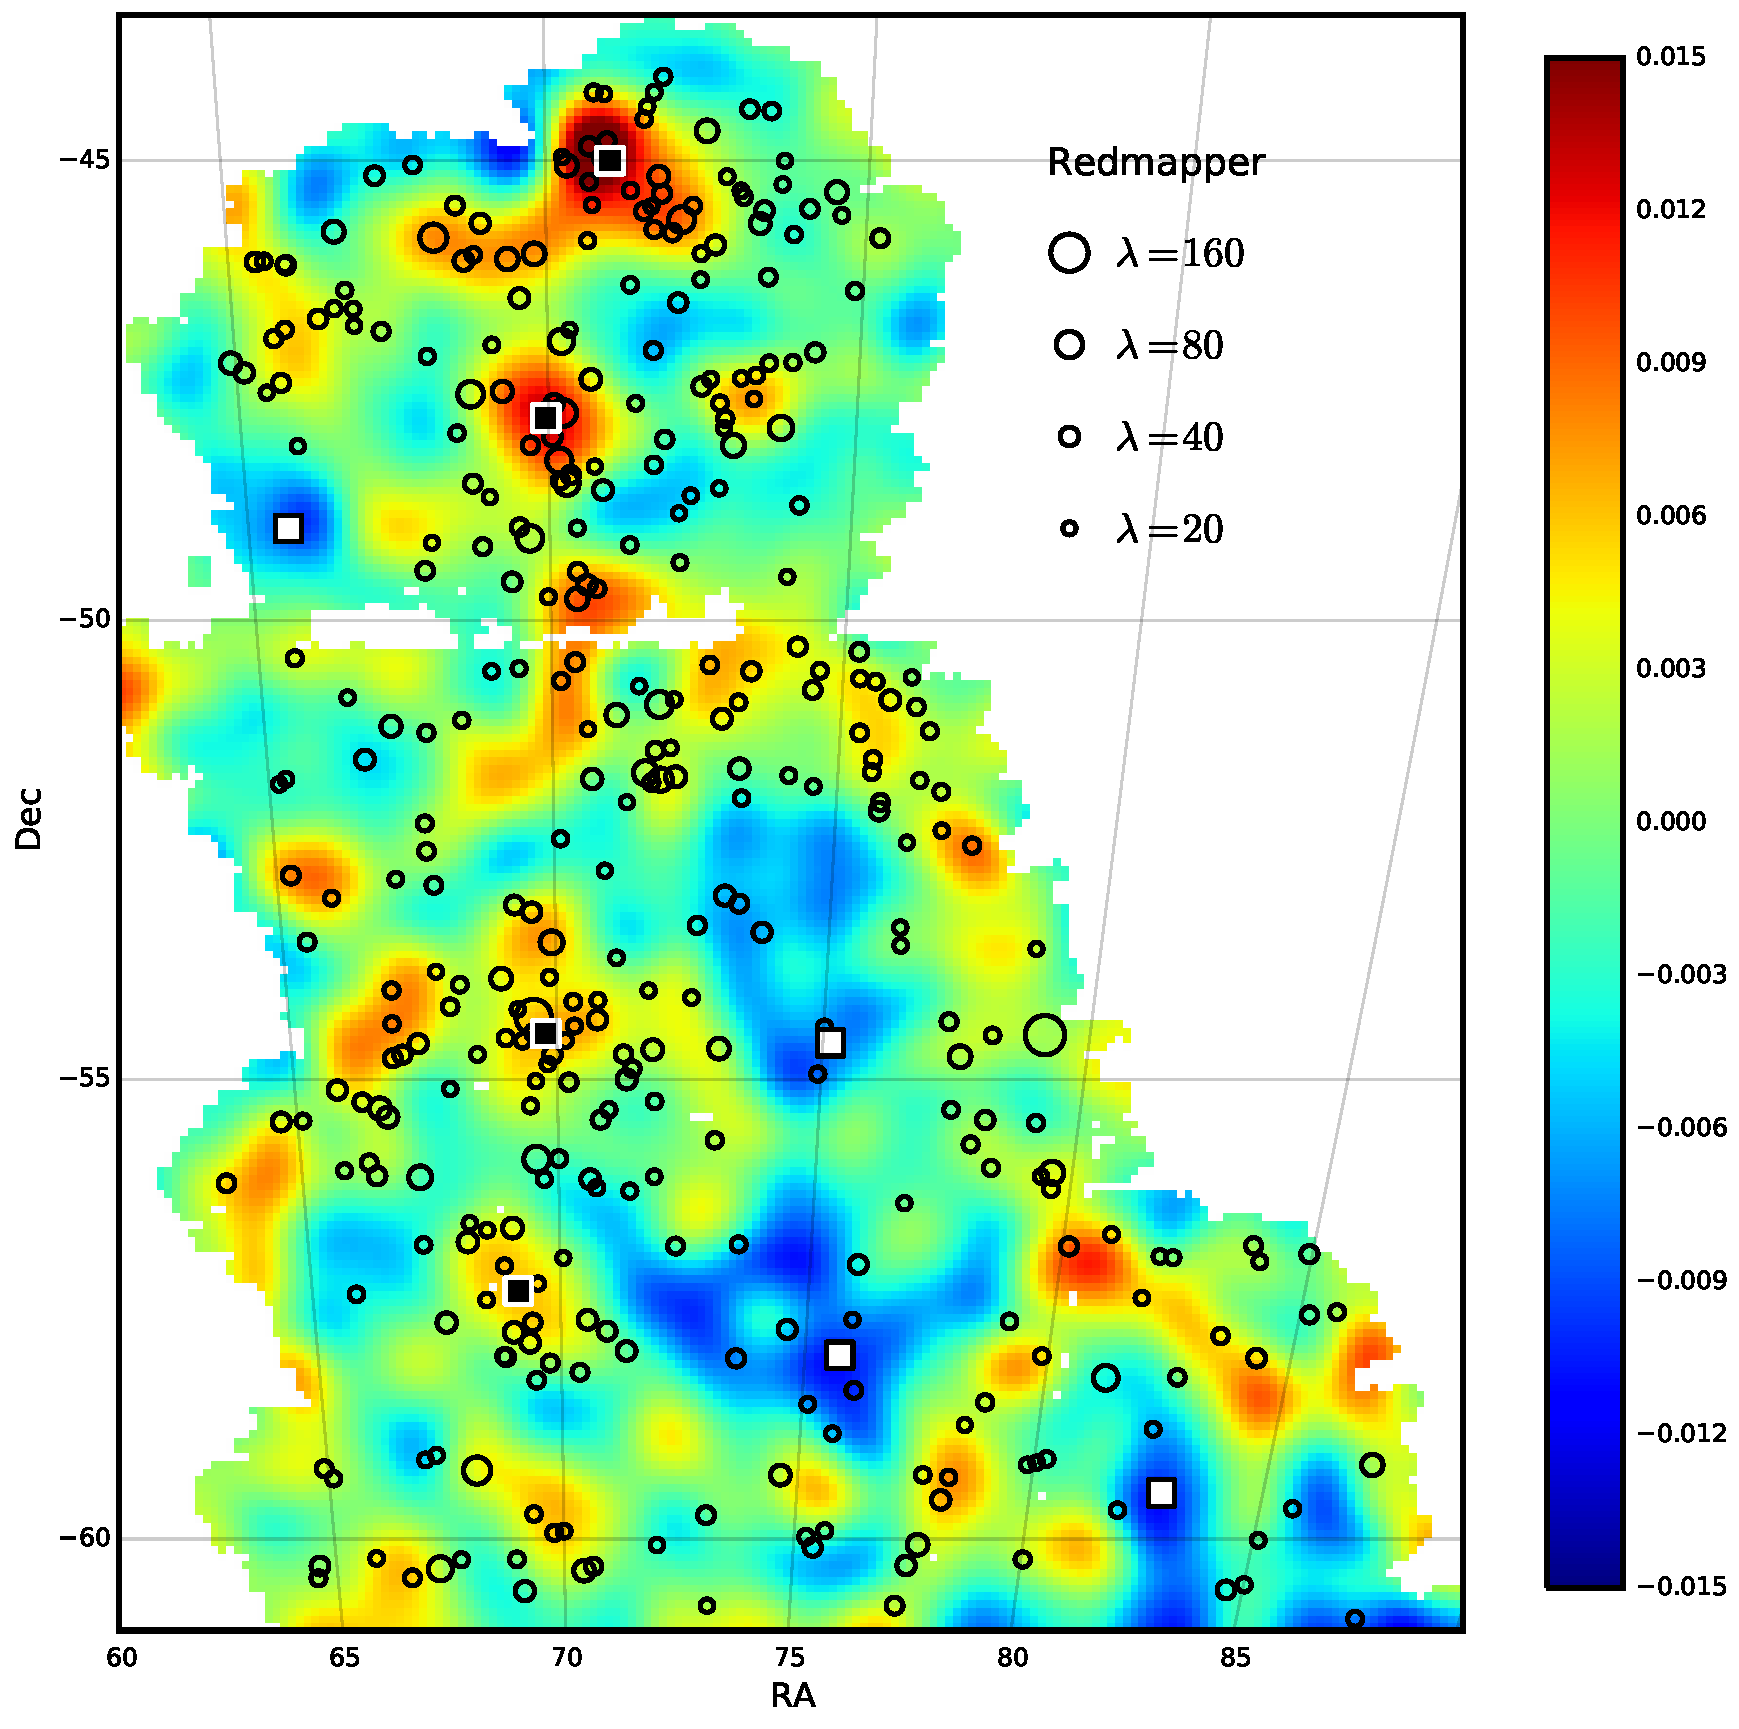
\includegraphics[scale=0.17]{cluster_overlay_ngmix_bpz.pdf}
            \newline
            {\tiny DES Mass Map, Vikram et al. 2015 PRD}
        \end{column}

    \end{columns}

}

\frame
{

    \frametitle{Dark Energy Survey}

    \fontsize{9}{0.8\baselineskip}

    \begin{columns}

        \begin{column}{0.5\textwidth}

            \begin{itemize}

                \item Sheldon was lead author, with Mike Jarvis, of the DES shear catalog
                    paper, as well as producing catalogs (Jarvis et al. 2016).  All
                    other lensing papers depend this work.

                \item E. Sheldon published, with Peter Melchior, a paper on the crowd
                    sourcing ``DES Exposure Checker'', used by DES scientists
                    to view and verify survey images (Melchior, Sheldon et al. 2015).

                \item Paper on lensing by clusters of galaxies, led by E. Sheldon,
                    now in final stages.  Part of the DES key project to constrain
                    cosmology from clusters and lensing.

            \end{itemize}

        \end{column}

        \begin{column}{0.5\textwidth}
            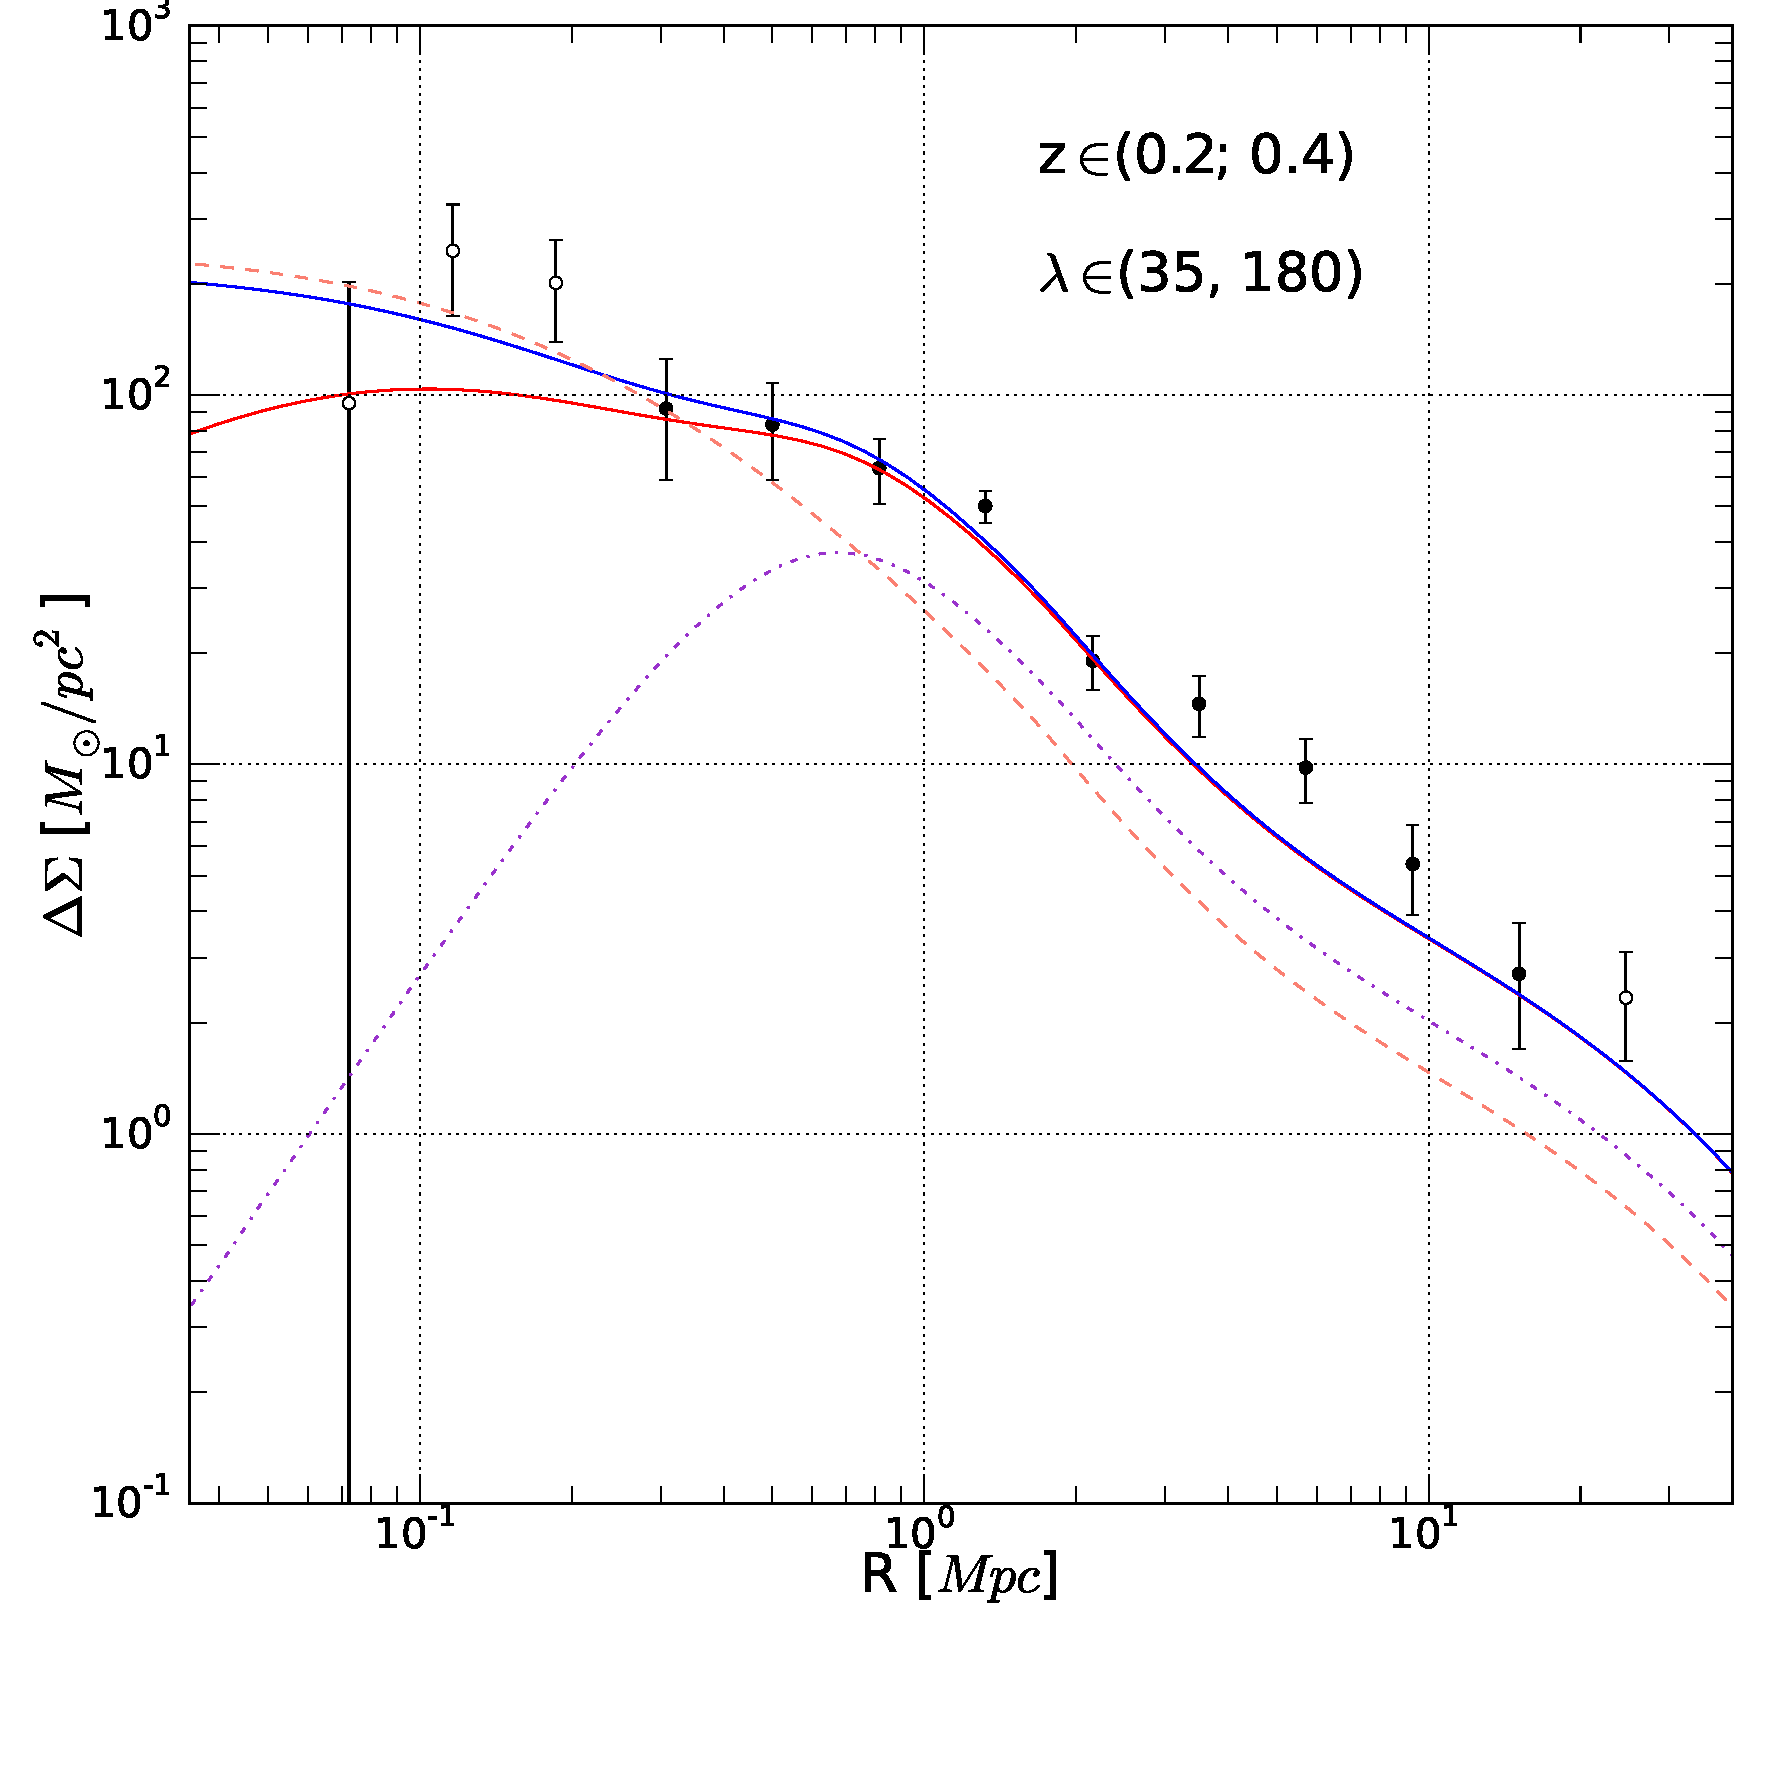
\includegraphics[scale=0.17]{delta_sigma_best_fit_z0_l4.pdf}
            \newline
            {\tiny Mass Density Constrast of DES Clusters. This figure is a placeholder.}
        \end{column}

    \end{columns}

}


\end{document}
